\documentclass[12pt]{TDTP}


\newcommand{\auteur}{Cedric Lemaitre}
\newcommand{\couriel}{c.lemaitre58@gmail.com}
\newcommand{\promo}{Bachelor in Computer Vision}
\newcommand{\annee}{2016-2017}
\newcommand{\matiere}{Digital Electronics}

\newcommand{\tdtp}{Practice}
\renewcommand{\sujet}{Digital Electonic simulation tools}


\begin{document}
\titre
We propose in this labs to create a tools to make to automatized the simulation and the understand of a logic function.
Use python language to create the following tools.
The tool is based on 2 major class : Wire and Gate.

\begin{itemize}
	\item Wire allows to connected component. Wire is connected on a unique output component and is connected on a multiple input component. 
	\item Gate contains function which describe behavior : AndGate, OrGate...
\end{itemize}

%%%%%%%%%%%%
\Exo

Create a class Wire with the following attributes :

\begin{itemize}
	\item a constructor (\_\_init\_\_)
	\item a method addDownstream which add a component addDownstream
	\item methods setState and getState which allow to manipulate state
\end{itemize}


%%%%%%%%%%%%
\Exo

Create some class for the gates : AndGate, OrGate, NotGate and XorGate. Each Gate have the following attributes :

\begin{itemize}
	\item a constructeur with input and output as parameters
	\item an update method
\end{itemize}
%%%%%%%%%%%
\Exo 

Create a class named Senser which is a special component (Gate).
This component have one input and one output. Its input is displayed each time that update function is called. 

%%%%%%%%%%
\Exo

Create a class Display which allow to display chronogram

\begin{figure}[h!]
\begin{center}
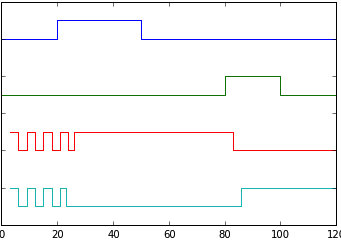
\includegraphics[width=.2\textwidth]{images/chrono.png}
\caption{Example of chronogram}
\end{center}
\end{figure}
%%%%%%%%%%

\Exo
Create a class which allow to realize the Karnaugh simplification

%%%%%%%%%%
\Exo
Try your software on the following function

\begin{figure}[h!]
\begin{center}
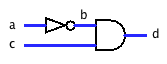
\includegraphics[width=.2\textwidth]{images/ex1.png}
\caption{Example 1}
\end{center}
\end{figure}

%%%%%%%%%
\end{document}
